\chapter{Design}\label{C:design}

The deign processes outlined within this report will draw heavily on the background research discussed in \Cref{C:background}. These designs aim to effetely implement the outlined system requirements in a robust and repeatable manner.


%
% SECTION Defining & Justifying System Specifications
%

\section{Defining \& Justifying System Specifications}\label{S:specs_design}

Based on the system requirements that have been outlined in \Cref{C:intro}, a set of system specifications can be created to inform our design decisions.\\

It has been specified that the final system design will be able to select for both the output load voltage, and the inductor current ripple of the buck converter. From this requirement we can identity that two separate control systems should be designed, one to regulate the output voltage of the converter, and one to regulate the inductor current ripple.

Next we can identify that to control the output load voltage and the inductor current ripple, we must be able to actively effect their current state. Based on \Cref{E:V_out} we can see that by varying the duty cycle of the converters PWM signal, we are able to directly control the output voltage. Similarly, from \Cref{E:delta_i} we can see that by varying the converters PWM switching frequency we are able to directly control the inductor current ripple. From this we can specify that our designs of the PWM generation must be capable of varying both the duty cycle and the switching frequency of the output PWM signal independently and simultaneously. \\

The outlined requirements also specify the level of precision that will be required from the output load voltage and the inductor current ripple. This allows us to specify the tolerable error for the system design, and calculate the minimum required system specifications. Based on the buck converter design equations from \Cref{S:buck_design_back}, The following specifications have been identified:

\begin{itemize}
    \item Maximum allowable duty cycle step size

    \begin{align}
        V_{error} &= V_{min} \cdot error = 0.15V\\
        D_{step} &= \frac{V_{error}}{V_{in}} = 0.0125\\
        N_{step} &= \frac{1}{D_{step}} = 80 \label{E:duty_step}
    \end{align}

    \item Maximum \& minimum inductor sizes

    \begin{align}
        L_{max}&=\frac{V_{max}\cdot\left(1-D_{max}\right)}{f_{min}\cdot I_{min}} = 27.7mH \label{E:L_max}\\ 
        L_{min}&=\frac{\frac{V_{in}}{2}\cdot\left(1-0.5\right)}{f_{max}\cdot I_{min}} = 0.5mH \label{E:L_min}
    \end{align}
    
    \item Maximum allowable frequency step size

    \begin{align}
        f_{step}&=\frac{V_{max}\cdot\left(1-D_{max}\right)}{\left(I_{min}-I_{Error}\right)\cdot L_{max}}-f_{min} = 52Hz\\
        N_{steps}&=\frac{\left(f_{max}-f_{min}\right)}{f_{step}} = 1881 \label{E:f_step}
    \end{align}

\end{itemize}

The derivation of these values can be found in \Cref*{A:specs}.

\subsubsection{TODO Refactor this to be a list of specifications}
From these equations we can build a list of final specifications to inform the design of our PWM generator and buck converter. The PWM generator must provide a minimum voltage step size of $0.0125$V, for a resolution of 80 voltage steps between 3V and 10V. The PWM generator must also be able to provide a minimum frequency step size of $52$Hz, for a resolution of 1881 frequency steps between $1$kHz \& $100$kHz. Finally we can also specify that the buck converter must be capable of functioning with inductor values between $0.5$mH \& $27.7$mH. \\

By designing the PWM generator and the buck converter to these specifications, we are able to guarantee that we can always achieve the requirements outlined in \Cref{C:intro}.\\

\subsubsection{TODO Discuss the minimum and maximum sense current, along with the bandwidth requirement of the sensors}
Design the system specifications around the current sensing and voltage sensing. What is the required bandwidth of the sensor? What is the required precision?\\


%
% SECTION System Architecture & Design
%

\section{System Architecture \& Design}\label{S:system_design}

To achieve the specifications that have been outlined in \Cref{S:specs_design}, it is important to design the system architecture around them. In \Cref{F:sys_overview} an overview of the system architecture can be seen, with three main design sections outlined. These sections each represent a significant segment of work that must be completed for the final artefact of this project to be achieved. \\

The first section of work that must be completed is the design of the PWM generation, denoted 1 in \Cref{F:sys_overview}. This PWM generator will be used to control both the output voltage and the inductor current ripple, and as such must be able to modulate both the duty cycle and the frequency of the PWM to the precisions required. \\

The second section of work is the design of the sensing elements required by the system, denoted 2 in \Cref{F:sys_overview}. These elements will be used to measure both the output voltage and the inductor current ripple, and therefore must be able to achieve the required precisions and sampling rates. \\

Finally the third section of work is the design and implementation of the two control systems, denoted 3 in \Cref{F:sys_overview}. These control systems will be responsible for maintaining the desired output voltage and inductor current ripple of the buck converter. This system will therefore be responsible for facilitating the final functionality of the project, combining sections 1 \& 2. \\

\begin{figure}[!h]
    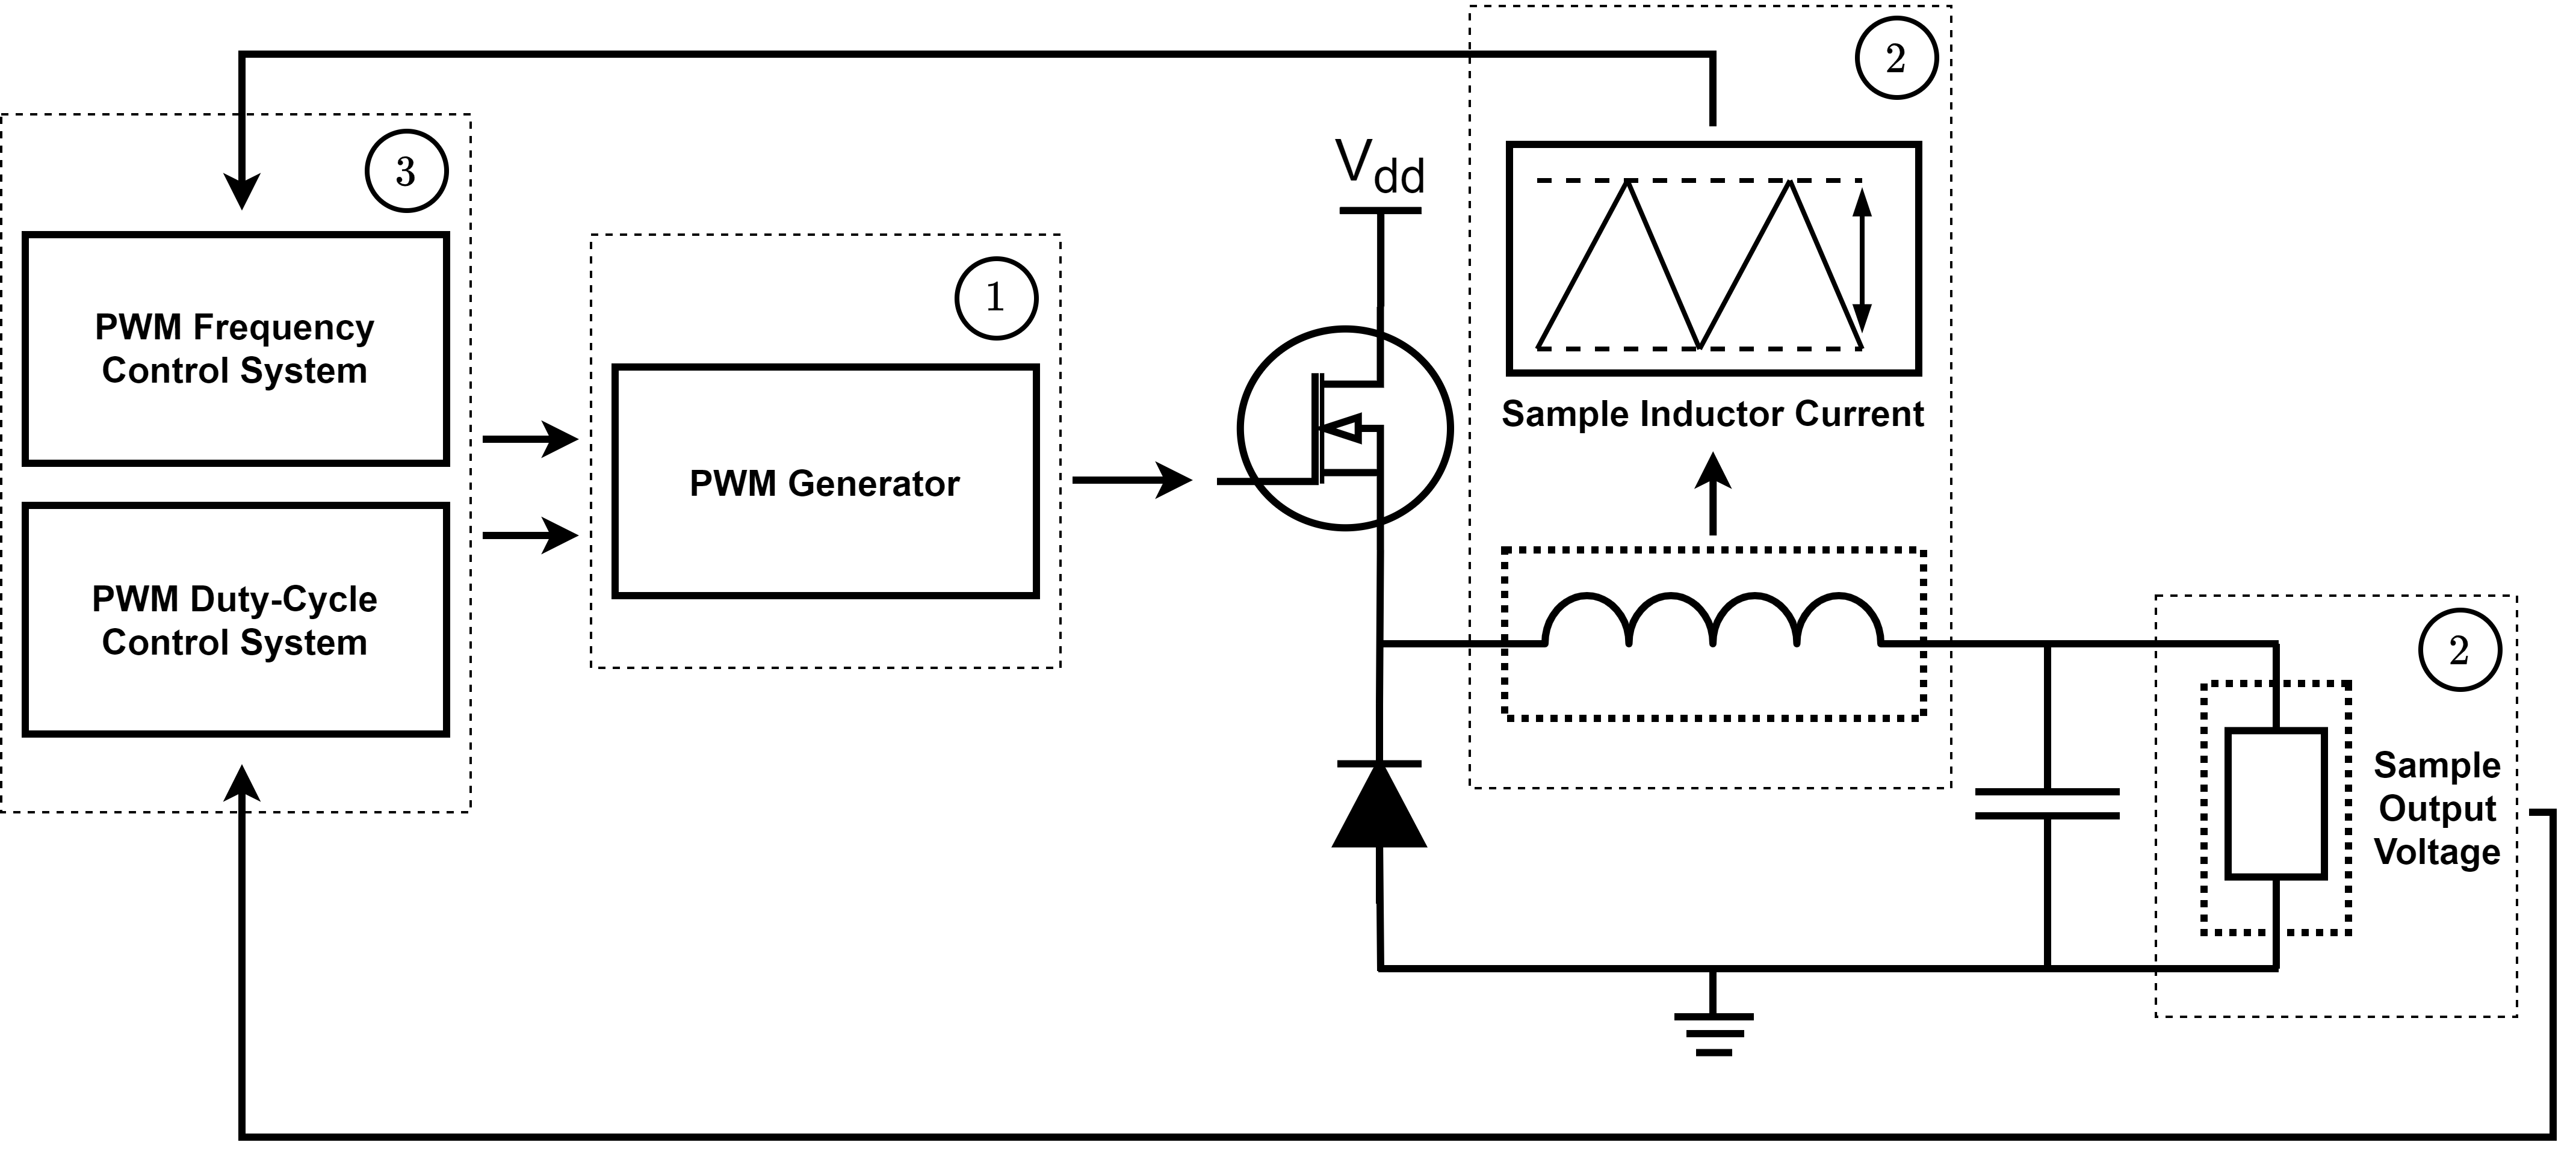
\includegraphics[width = \textwidth]{System_Overview.png}
    \caption{High level system overview}
    % \vspace{-20pt}
    \label{F:sys_overview}
\end{figure}


%
% SECTION PWM Generation
%

\section{PWM Generation}\label{S:pwm_gen_design}

In the design of the PWM generator, both the analogue and digital designs discussed in \Cref{S:PWM_back} were considered, designed, and tested for. Each of these designs presented pros and cons that would affects the overall design of the system architecture. This section will discuss these designs and finalise the design of the PWM generator for this system. 

\subsection{Analogue PWM Generator Design}\label{S:PWM_analogue_design}

As discussed in \Cref{S:analogue_PWM_back}, the design of the analogue PWM signal generator requires three stages, each of which will have its own design requirements based on the specifications outlined in \Cref{S:specs_design}. \\

The clock generation stage will be responsible for setting the frequency of the final PWM signal. This specifies that the clock source have a variable frequency output range between $1kHz$ and $100kHz$, with a minimum step size of $52Hz$. Research was done on a variety of clock sources, looking at voltage-controlled oscillators (VCO's), signal generator IC's, and even the basic 555 timer. From this VCO's were identified to operate at much higher frequencies than those used in this project. It was also identified that signal generator IC's often require selections of passive components to operate effectively, increasing their complexity. For this reason the variable frequency 555 timer circuit was selected, as it provided the required specifications.\\

The next section designed was the signal integrator stage. This stage consisted of a basic op-amp integrator circuit, with a design requirement that it be able to integrate the clock signal across the frequency range required. This circuit was designed and implemented in an LTSpice simulation to evaluate it's performance, and can be seen in \Cref*{A:analogue_PWM}. From this simulation it was noted that the integrator's frequency response was similar to that of a first order low pass filter, and greatly attenuated the integrated signal. For this reason it was decided that analogue PWM generation would not be implemented in this system, as it presented many issues.

\subsubsection{TODO insert images of the designed integrator circuit, and it's frequency response (bode plot)} 

\subsection{Digital PWM Generator Design}\label{S:PWM_digital_design}

As discussed in \Cref{S:digital_PWM_back}, The design of the digital PWM generator is far simpler than that of the analogue, and can be implemented in a wide variety of methods. In this project microcontrollers and FPGA's have been considered.

Based solely on the capabilities of the platform, the PWM generator would be best designed and implemented on an FPGA as it would allow for superior speed and precision. However FGPA design brings a lot of difficulties, primarily in the prototyping and testing stages. Because of this, due to the limited time from of this project, we have decided to implement this PWM design using a microcontroller.

The selection of the microcontroller is highly dependant on the clock frequency and design of the PWM peripherals, as it must be capable of achieving the specifications outlined in \Cref{S:specs_design}. A large selection of microcontroller data-sheets were reviewed to identify their specifications, including AVR, STM8, Espressif, and teensy based microcontrollers. From this review it was decided that the ESP32 microcontroller would be best suited to this project \cite{ESP32Manual}. This microcontroller is capable of outputting a maximum PWM frequency 125$kHz$ with a duty cycle resolution of 9 bits (512 voltage steps). From here a short C program was written to test the PWM functionality of the ESP32, and it was confirmed that it met the required specifications. The source code and images of this PWM signal can be found in \Cref{A:digital_PWM}.
 

%
% SECTION Inductor Current Ripple Sensing Design
%

\section{Inductor Current Peak to Peak Sensing}\label{S:current_sense_design}

Discuss the purpose of this sensors, and the requirements of the sensing system in regards to its range, precision, and bandwidth. Also discuss the required outputs of the sensor (we need to detects the current peak value, and the mean current).


\subsection{Current Sensor Selection}\label{S:current_sense_selection}

Talk about how hall effect sensors were identified to not be suitable for this design due to the reasons outlined in \Cref{S:hall_effect_back}. From here the discuss the selection of a current sense amplifier (it's gain, bandwidth, and precision), and then the selection and design of the shunt resistor. Then discuss the expected voltage output of this current and the expected waveform. 


Based on the specifications outlined in \Cref{S:specs_design}, it can be identified that directly sampling the output waveform from this sensors is not feasible due to it's large possible bandwidth. From there then discuss the design of varying analog circuits to attempt to identify the peak current and mean current. 

I want to show circuit designs, and simulations for both the precision rectifier peak detection design, and the capture and hold peak detection design. 

\subsection{Precision Rectifier Peak Voltage Detection}\label{S:current_sense_precision_rectifier_design}

Design, and simulations of the Precision Rectifier Peak Voltage Detection.

\subsection{Sample and Hold Peak Voltage Detection}\label{S:current_sense_sample_and_hold_design}

Design, and simulations of the Sample and Hold Peak Voltage Detection.

\subsection{Current sensing digitisation}\label{S:current_sense_ADC_design}

Discuss the selection of the ADC for measuring the peak ripple and mean ripple currents. Talk about the minimum required ADC precision, and bandwidth requirements.  


%
% SECTION Control System Design
%

\section{Control System}\label{S:control_design}

The control system designs will inform the selection of the sensors used within the system design. This section will cover the selection of the controller topology (PI \& PID), some basic modelling of the system, and then the selection of the sensors required to generate the correct feedback signals. 

\subsection{Output Load Voltage Controller}\label{S:output_control_design}

\subsection{Inductor Current Ripple Controller}\label{S:ripple_control_design}





